\chapter{Creating Machine Learning Model}
\label{chapter:4}

\section{Observed Systems}
\label{section:4.1}

\subsection{Water Molecule H2}
\label{subsection:4.1.1}

The first observed and analysed system consists of  two Hydrogen Atoms forming a Molecule. $H_2$ is pictured in cartesian coordinates in \ref{fig:H2VMD}. The atom configurations stem from a \textit{Molecular Dynamics (MD) Simulation} computed using Density Functional Theory. The Hydrogen Atoms in the Simulation are fixed in the \textit{x-y-plane} and oscillate in z-\textit{direction}. 

With the system only changing in distance between the two hydrogen atoms, building a \textit{Machine Learning model} using a  two body distance abbreviation, presented  in \ref{subsection:3.3.4}, is sound. The atoms oscillate in one dimension with no changes in angle between them, making a two-body descriptor taking only the distance between them into account suitable. 

\begin{figure}
	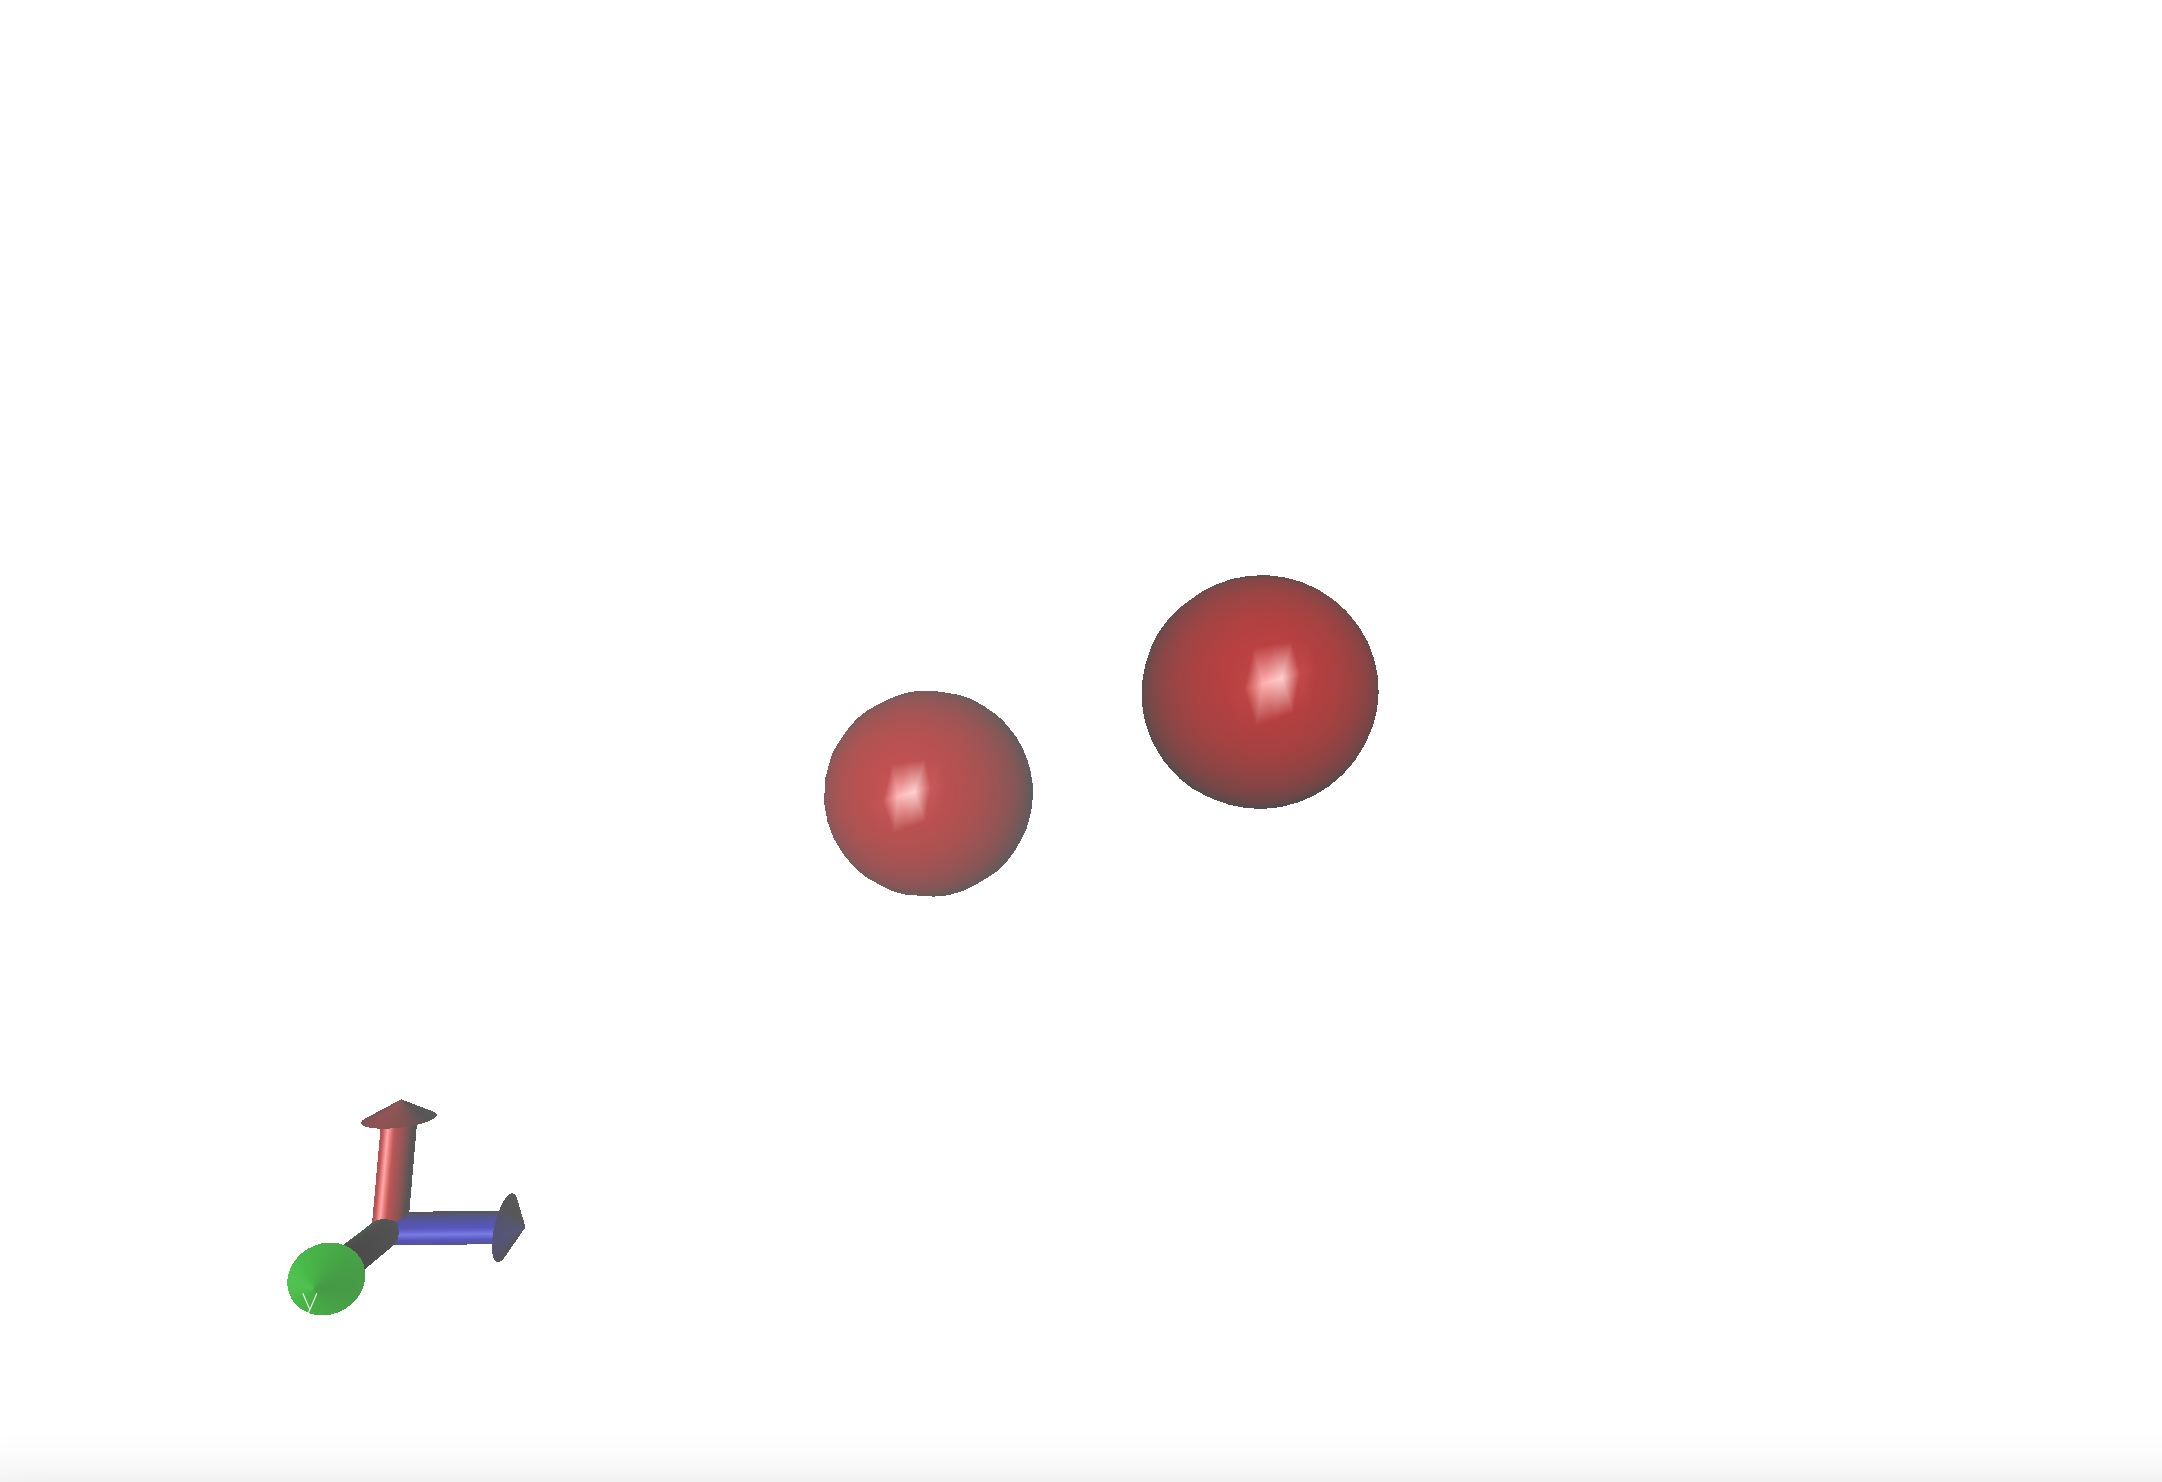
\includegraphics{../Bilder/Hydrogen_Tuple_Fig1.png}
	\caption{$H_2 Molecule$}
	\label{H2VMD}
\end{figure}


\subsection{Water Crystal}
\label{subsection:4.1.2}
Second, a a larger more complex system of a \textit{Hydrogen Crystal}, containing 192 Atoms is introduced. Again the atom configurations are the output of a \textit{Molecular Dynamics (MD) Simulation} computed quantummechanically making use of the Approximations of \textit{DFT}. For simplicity reasons a \texit{MD} is run for a bulk of atoms of just one type. The way the software, to create the \textit{ML-Model}, is built this  simplicity restriction could be lifted and the system could be updated to include multiple atom species.

The Hydrogen\textit{H} in form of a crystal is depicted in \ref{fig:HCrystalVMD}. The \textit{MD} run to generate the atomic configurations starts at a state of atoms out of ground state. Running the Simulation and generating the training data for the model the atoms then relax to an equilibrium state. The atomic configurations yielded each time-step serve as as basis of the building process of the \textit{Machine Learning Model}.  

To describe this system, again a pairwise distance descriptor is used. The two body descriptor oversimplifies the problem and there is a loss of information describing a 192-Atom \textit{Hydrogen Crystal}. This is done to compare results of the same \textit{Machine Learning Algorithm} for two systems of differing complexity. 

\begin{figure}
	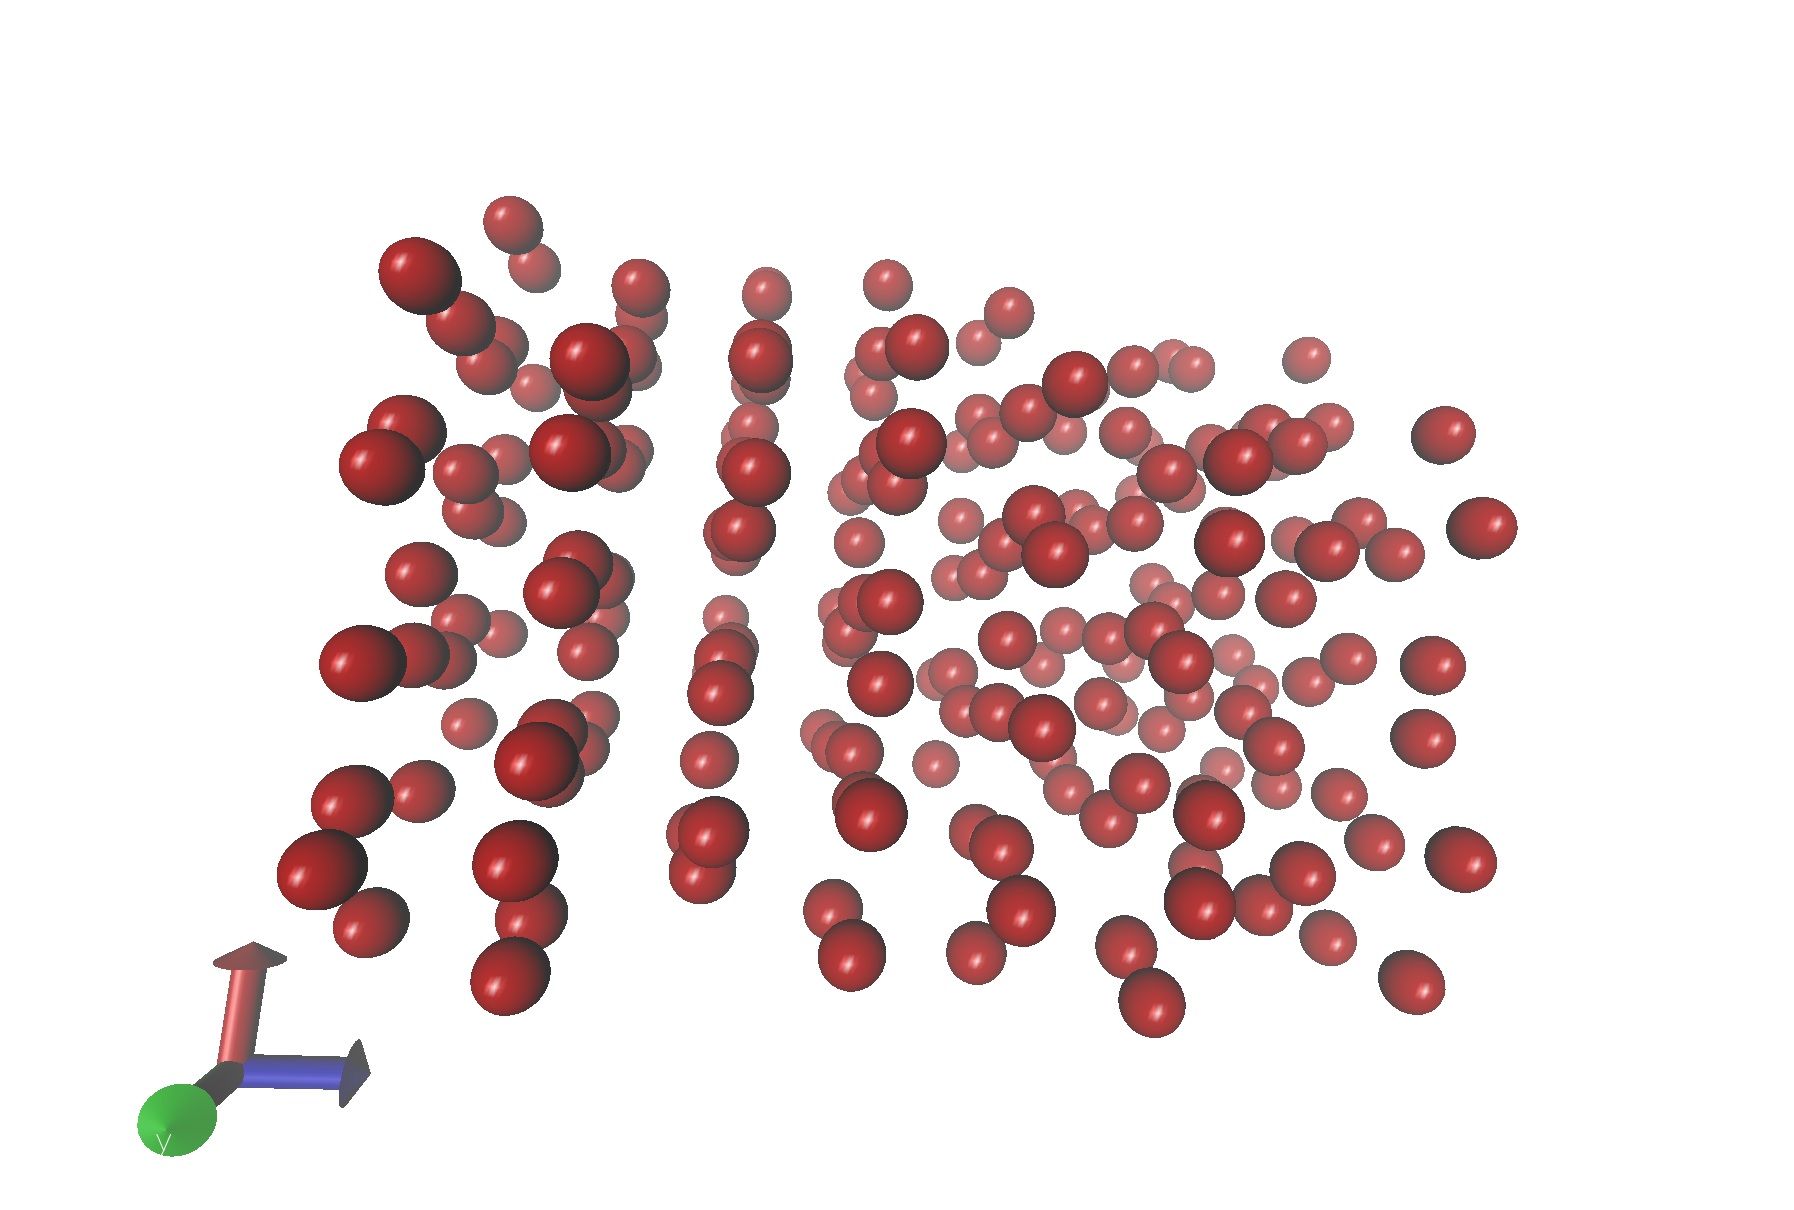
\includegraphics{../Bilder/Hydrogen_Crystal_Fig1.png}
	\caption{Hydrogen Crystal}
	\label{HCrystalVMD}
\end{figure}



\section{Workflow, making a model, use H2 as example}
\label{section:4.2}

\subsection{Flow-Chart, steps are explained in further detail in the following chapters}
\label{subsection:4.2.1}


Creating the \textit{ML-Model} is not a linear process, but a circular one. As can be seen in the Flowchart \ref{fig:flowchart} there are several steps building the model and turning the process into a result optimising feedback loop. The depicted Flowchart lays the foundation for creating and tuning the model and its steps are derived in the following chapters. 

\begin{figure}
	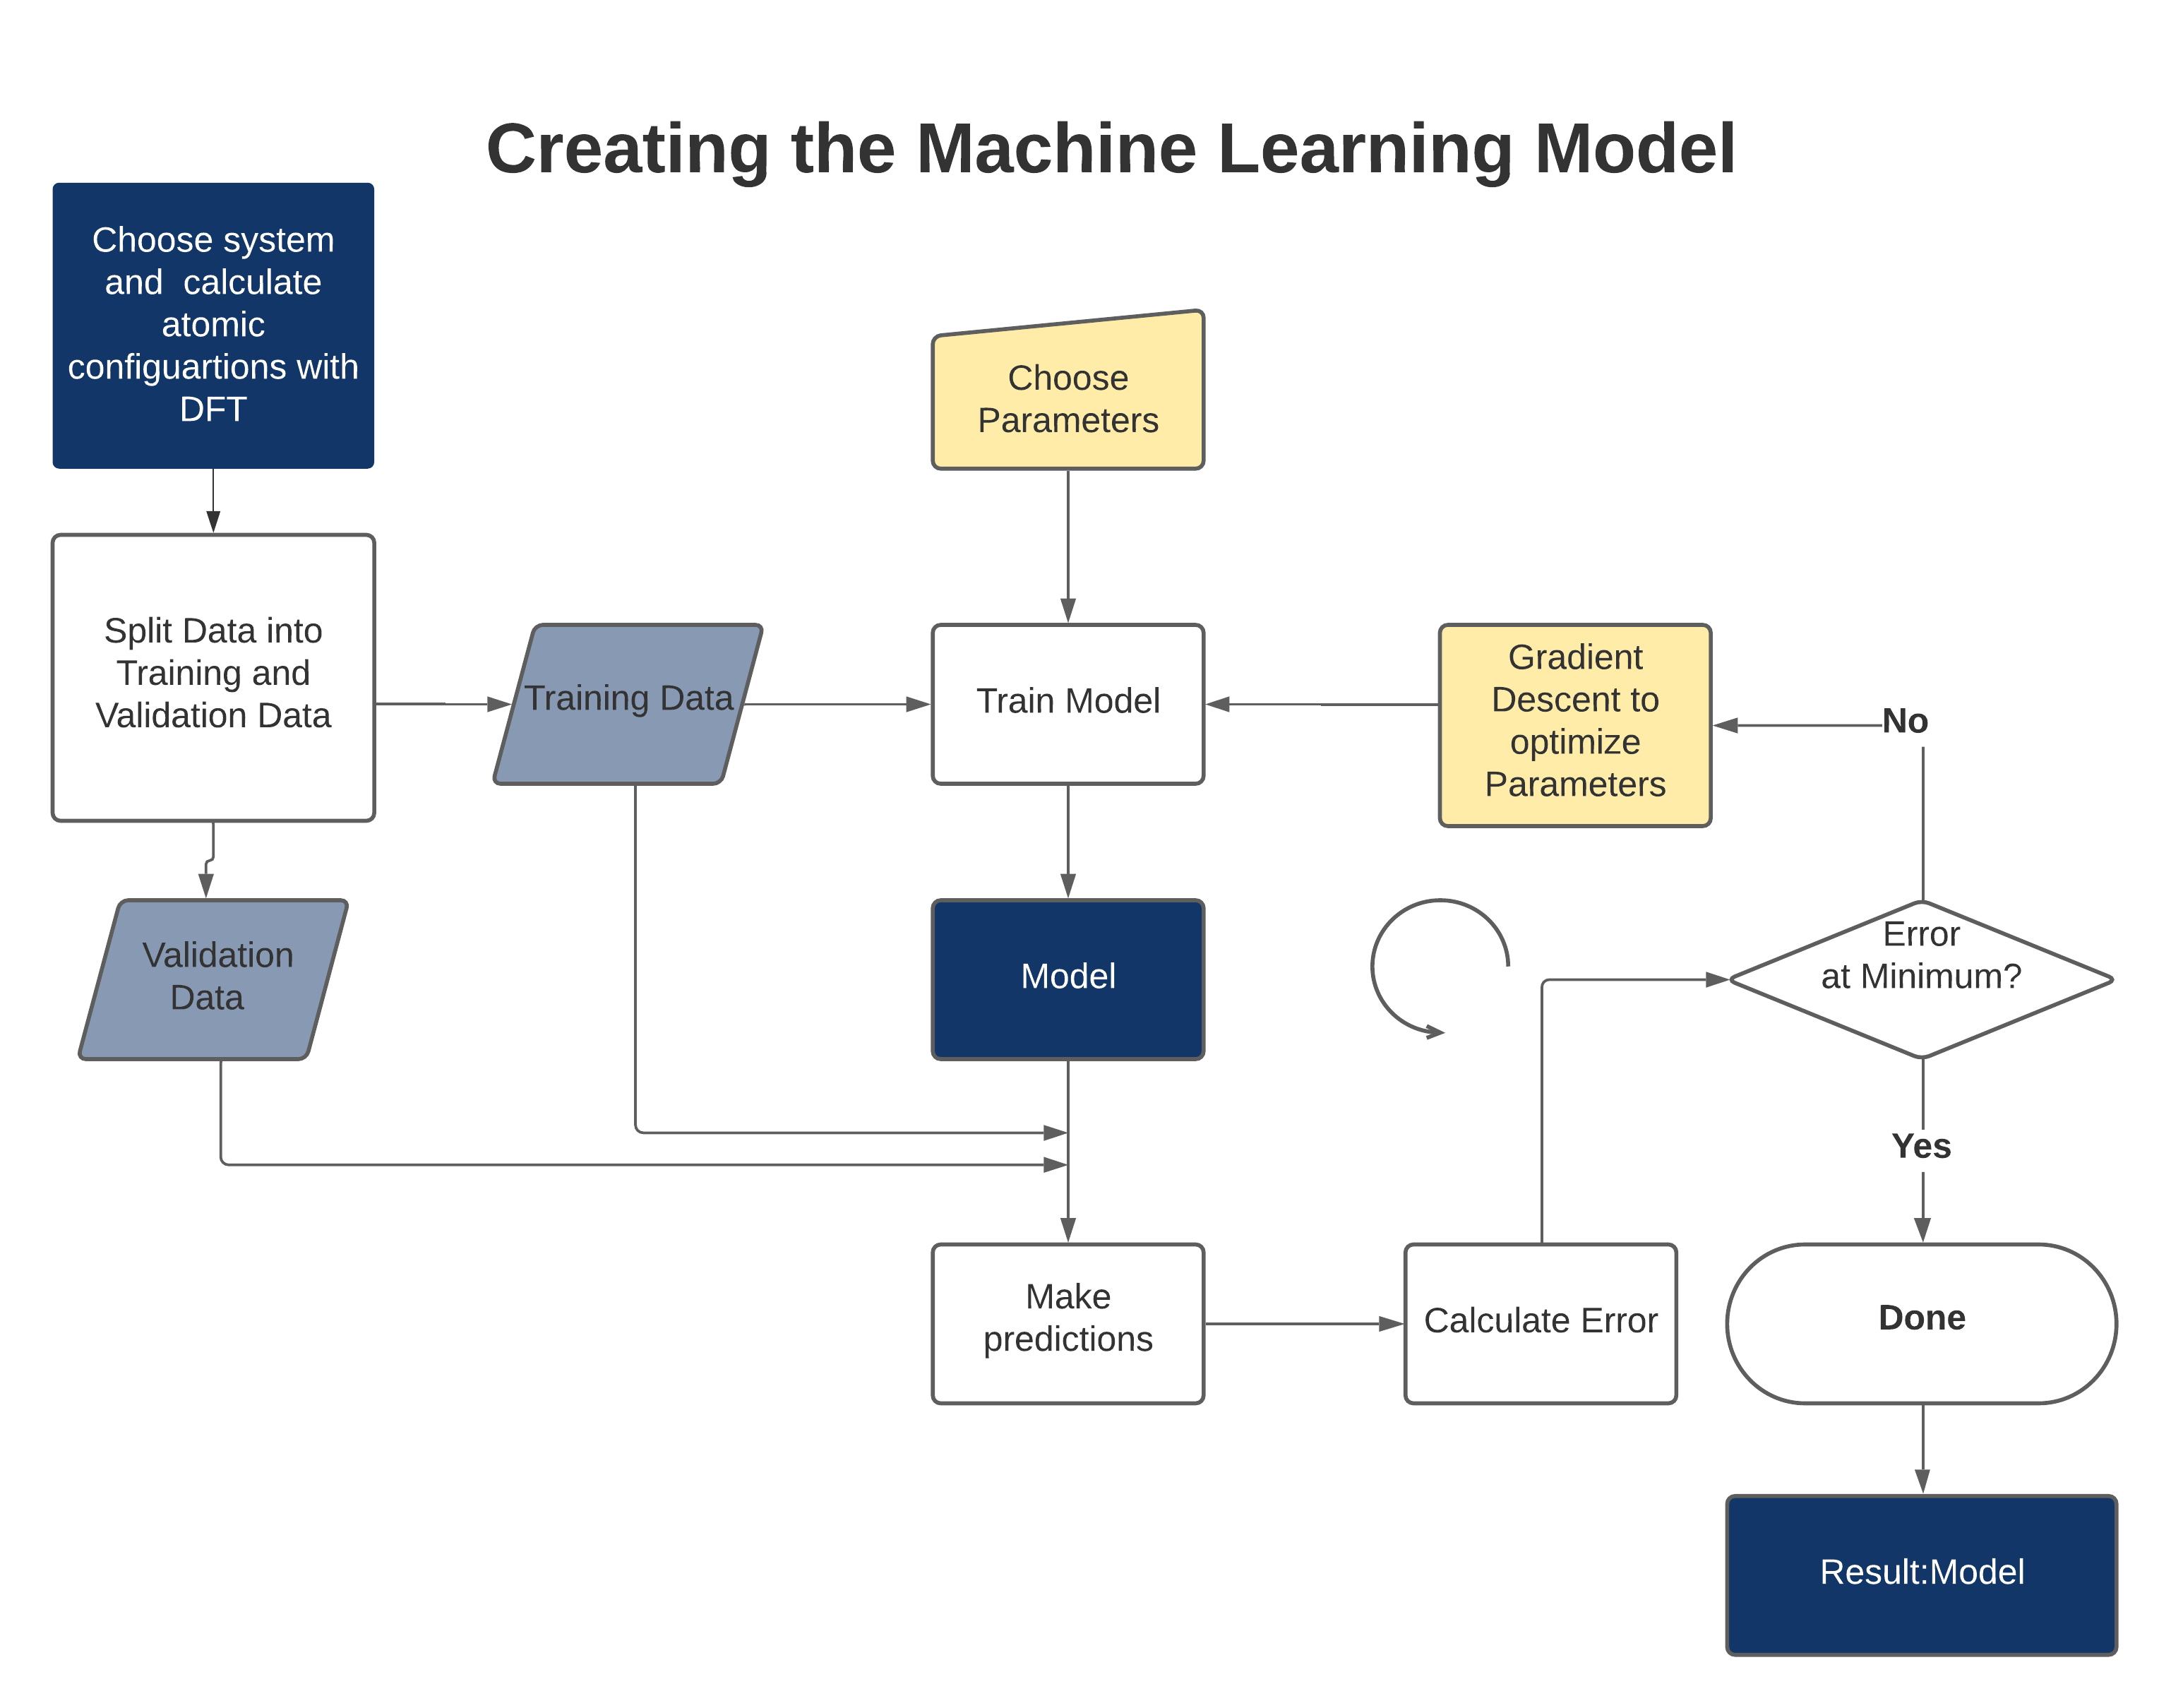
\includegraphics{../Bilder/Flowchart_ML_Model.png}
	\caption{Flowchart of Creation of the Machine Learning Model}
	\label{flowchart}
\end{figure}

\subsection{Get Data from DFT}
\label{subsection:4.2.2}

Beginning at the top of the Flowchart the first step on the way to creating a model is choosing which system is going to be modelled and then run a \textit{Molecular Dynamics Simulation}, briefly explained in \ref{section:4.1}. The simulation uses \textit{DFT} to yield atomic configurations for each time step, these serve as input to the model. Details on how DFT solves quantummechanical problems are derived in chapter \ref{chapter:2}. The following chapter explain the workflow to go along with the flowchart on the example of the system containing the \textit{H_2 Molecule}. The \textit{MD} outputs a a set of atomic constellations with a corresponding energy per constellation and an associated force for each atom of the system per constellation. The data then needs to be transformed from an \textit{.xml} file coming out of the \textit{MD} to a certain file format, namely an \textit{.xyz} file so it can be interpreted correctly by the software used to create the model. Details are derrived in the Appendix. TODO: reference correct letter of apendixx


\subsection{Split Data into training and validation Data}
\label{subsection:4.2.3}

It is good practice in any \textit{ML-process} to split up the input data into two parts.  \footcite[17]{intro-ml} One is going to be the training data used, directly used in the model building process and the other part is saved to evaluate and improve the model, that is validation data. Once the model has gone through the first iteration of its optimisation loop the validation data is used to see the quality of the model. This is  done by letting the model make prediction on the validation data it has not been trained on. Saving a part of the input data for validation is done to prevent the model from overfitting, by using the validation data to refine the model. Overfitting means the model is highly accurate on reproducing the results of the training data but fails to correctly classify new input data.  

In this case the split up between the training and validation data is done randomly and the ratio of the fit is set to $0.8$. An $0.8$ ratio delegates 80 percent of the input data for the model to training data and marks 20 percent as validation data. The ratio is by choice, but the way the code is written for this work it is possible to change split percentages and construct the model with a different split. 

(TODO: maybe create simple pie chart for split - training data, validation data)

\subsection{Input Data to ML Model - Train Model}
\label{subsection:4.2.4}

Following the split into training data and validation data, the latter is put aside and the training data is input to the \texitit{ML Process} which uses Gaussian Process Regression as underlying tool. Details are derived in chapter \ref{chapter:3}. The algorithm works like a black box where pairs of atomic configurations and the associated energies and forces are input to the model. In addition a set of parameters is demanded due to the algorithmic of the Gaussian Process. There are parameters true to the nature of the Gaussian Process and further descriptor specific parameters. The chosen descriptor here is the \textit{2-body-distance}. The black box model is trained, meaning in builds instructions by internally setting certain variables to certain  values, which then enables the model to predict atom energies and forces for given atomic constellations. 

The required parameters by the Gaussian Process represent the expected variance $\sigma$ of the training data. \footcite[Appendix]{GAP-2009} Intuitively this can be thought of as intrinsic noise of the training data. Mathematical details can be found in \ref{section:3.2}, 
\begin{itemize}
	\item $\sigma_E$, variance of training data energies 
	\item $\sigma_F$, variance of training data force 
	\item $\sigma_S$, variance of training data functional derivatives of energies, this is the virial stress  \footcite[1053]{GAP-intro} 
	\item $\sigma_H$, variance of training data  functional second derivatives of energies, this is the hessian \footcite[1053]{GAP-intro} 
\end{itemize}

The 4 $\sigma $ parameters are the diagonal elements of a \textit{variance} matrix. 


The \textit{2-body-distance} descriptor requires the following parameters to be set, details can be found in \ref{section:3.3}: 
\begin{itemize}
	\item Cutoff radius, sets geometrical distance for each atom up to which its environment is considered by the model, in \AA ngstrom 
	\item Covariance type, sets how the kernel is built using the descriptor transformations of the input data as basis functions
	\item $\theta$, goes into the computation of the covariance type as denominator. Determines the "size" of the classification bins by resembling the geometrical scale of the input data.
	\item $\delta$, puts weight on the kernel for the chosen descriptors if there is more than one. The input settings determine the choice of  $\delta$. 
	\item Sparse method, sets the method the sparsification is performed. The sparse data is  a representative selection all the input data
	\item Number of sparse points, defines the magnitude of the reduction on the sparse point set
\end{itemize}

Of the needed parameters an educated choice is made for all but $\sigma_E$ $\sigma_F$ and $\theta$, those are later optimised using a Gradient Descent Method. The predetermined parameters are set to the following values:

\begin{itemize}
	\item Cutoff radiu: 4 \AA ngstrom
	\item Covariance type: Squared Exponential \footcite[Appendix 2.1.]{GAP-2009}, see \ref{eq:kernel} 
	\item $\delta$: 1, can be set to any value due to just one descriptor being used, hence no no weighting between different descriptors is needed
	\item Sparse method: Uniform, this means the sparse points are chosen based upon a selection of bins all of the same size. The size of the bins is determined by a uniform grid. \footcite[2]{sparse_uniform}
	\item Number of sparse points: 20, for the $H_2$ System this is redundant and means all the atoms, but for the 192 Atom $H-Crystal$ the sparse representation is relevant
	\item $\sigma_S$: 0.0 
	 \item $\sigma_H$ 0.0 
\end{itemize}

\begin{equation}
	\label{eq:kernel}
		C(x_n,x_m) =
		\delta^2
		exp
		\left(
			-\frac{1}{2}
			\frac
			{(x_n-x_m)^2}
			{\theta^2}
		\right)
\end{equation}

\begin{itemize}
	\item $C(x_n,x_m)$ ... kernel, covariance matrix between two configurations
	\item $\delta$ ... weighting between different descriptor 
		kernels
 	\item $x_n$ ...descriptor value of $n_th$ configuration
	\item $x_m$ ... descriptor value of $m_th$ configuration
	\item $\theta$ ... hyperparameter, weighs the scale of input configurations
\end{itemize}}


Note that the variance of the virial stress and the hessian in the training data are set to zero because no further deviation for the derivation is expected. This is due to the \textit{2-body-distance} descriptor operating in one dimension. 
Choosing the fixed parameters is done based upon knowledge of the analysed atomic system. Varying the "fixed" parameters will not result in a recognisable change of the model. Thus not further optimising them is reasonable in respect to its cost. 

The most dependencies on the quality of the model rely on $\sigma_E$ $\sigma_F$ and $\theta$. It turns out that applying an optimisation algorithm to them returns the most precise results and converges fast to an optimum in fit. Still a guess needs to be made for 
 $\sigma_E$ $\sigma_F$ and $\theta$ to then pass to the first iteration of the cyclic optimisation process. A first guess is made:
 
 \begin{itemize}
	\item $\sigma_E$: 0.004 $eV$
	\item $\sigma_F$: 0.08 $\frac{eV}{\AA ngstrom}$
	\item $\theta$: 1.0 
\end{itemize}
 
 Note that it makes sense to select the variance of force to be one order lower as the variance of energy, since calculating forces includes derivatives which propagate the error and amplify it. (Is this true?)
  
 Following the flowchart in \ref{subsection:4.2.1} the model can enter the optimisation process with the input of: 
 
 \begin{enumerate}
 	\item Training data consisting of atomic configurations with their corresponding energies and forces 
	\item Set of fixed and variable parameters 
\end{enumerate}


\subsection{Make predictions}
\label{subsection:4.2.5}

Using the model to make predictions requires any set of atomic configurations as input and gives a set of energies and forces as output. If the output values resemble the values of a quantum-mechanical computation using, for example, \textit{Density Functional Theory}, then the model is correct. In detail the prediction yields one energy per atom configuration and forces for each atom for each spatial coordinate per atom configuration.

Going back to the flowchart in  \ref{subsection:4.2.1} the prediction is performed on the training data and additionally on the validation data. This is done to see how the model fares on input it has not been trained on. The mathematical details on how the prediction is performed based on the input data and the chosen parameters is derailed in chapter \ref{chapter:3}. 

\subsection{Optimise Process by minimising Error}
\label{subsection:4.2.6}
The model is trained and able to make predictions. To optimise the quality of the model a measure of goodness is needed. The error, in this case the \textit{Root Mean Squared Error (RMSE)}, is used as measure of inverse goodness. The \textit{RMSE} is a measurement of how fare the predicted values are off compared to the real values. A perfect model would always predict values mirroring real values, barring any intrinsic inaccuracies in the data, leading to an \textit{RMSE} of zero. Then \textit{Root Mean squared error} is a highly simple measure of error as it just takes the root of the mean of the squared error of two values: 

\begin{equation}
	\label{eq:RMSE}
		RMSE = \sqrt{
		\sum_{i=1}^{N}
		\frac
		{(\hat{X_i} - X_i)^2}
		{N}
}
\end{equation}

The denotations in \ref{eq:RMSE} are

\begin{itemize}
	\item $\hat{X}$ ... predicted value 
	\item X ... real value
	\item N ... number of real and predicted value pairs
\end{itemize}


Further computational details are explained in \cite{RMSE}.


In general a model is considered valid if it performs well but not perfect on the training data. A perfect resemblance of the training data would lead to overfitting and to inaccurate predictions of new, unknown input data. The validation data comes into place as it is unknown input data for the model. For both, the training atomic configurations and validation atomic configurations, the associated energies and forces are known. In this case \textit{real} means calculated by \textit{DFT}, which is assumed to mirror the features of a real system precisely bewaring numerical errors. To measure  the quality of the fit, the trained model is used to make calculations on the training data and validation data and output the related energies and forces. The output is then compared to the real values of energies and forces by calculating the \textit{RMSE} between them. This is done by calculating the \textit{RMSE} for every real value, predicted value tuple and then added up. The summarised error is then proportional to the difference between the real energies and forces and predicted energies and forces. 

A small \textit{RMSE} means predicted and real values lie close to each other. This is a good fit and the model works correctly. To get a well performing model the training, predicting and calculating the error procedure is plugged into a cycling optimisation algorithm. Since the atomic configurations cannot be changed the goal of the optimisation is to minimise the \textit{RMSE} by tuning the model parameters, namely  $\sigma_E$ $\sigma_F$ and $\theta$. The optimisation is done by a Gradient Descent Method. The \textit{Nealder-Mead Downhill Simplex Algortithm} is used to minimise a function, to which  $\sigma_E$ $\sigma_F$ and $\theta$ are passed as independent arguments and and the \textit{RMSE} is output as dependent variable. The dependent variable is the one to be minimised. Details on the \textit{Nealder-Mead Downhill Simplex Algortithm}, can be found in \cite{nealder-mead}.

For this work, the built in python package \textit{scipy} is used to minimize the \textit{RMSE} . An example function call  for the optimisation of \textit{H_2} can be seen in the code snippte below. Details can be found in the appendix \ref{chapter:6}. (TODO: get right appendix letter for scipy).

\begin{lstlisting}
import scipy.optimize
initial_guess = [1,0.004,0.08]
result = scipy.optimize.minimize(RMSE_train_val,initial_guess,method='Nelder-Mead',
                                 options={'fatol':10e-5,'maxiter':100})
\end{lstlisting}

The following arguments are passed to the optimisation algorithm: 

\begin{itemize}
	\item \textit{RMSE_train_val} is the function to be minimsed
	\item \textit{initial_guess} for the parameters $\sigma_E$ $\sigma_F$ and $\theta$
	\item \textit{fatol} is an exit condition for the algorithm, once the \textit{RMSE} converges to a minimum with and converges with \textit{fatol}, the process is stopped.
	\item \textit{maxiter} is an exit condition for the algorithm. If the optimisation process exceeds the number passed to \textit{maxiter} it is terminated
\end{itemize}

Notice that the contribution of the \textit{RMSE} of every real value, predicted value pair of energies and forces need to be scaled and cannot simply be added up and passed on to the minimiser. This is due to the ratio between the energies and forces for each configuration. Each atomic constellation hold energies for the whole system at a specific point wheres forces are attached to every atom of the constellation for every spacial coordinate at a specific point. Referring to the $H_2$-molecule of the \textit{MD-simulation} this means one energy for each time step compared to 6 forces, two atoms and three cartesian coordinates. 

To scale the \textit{RMSE} contributions correctly and to provide easy comparability to different atomic systems a per atom \textit{RMSE} is introduced. In General, for any system, this is done by dividing both, the energies and the forces by the number of atoms ind the configurations. Additionally the Forces need to be divided by the number of spatial coordinates, for cartesian systems this means dividing by three. The scheme is shown in \ref{eq:RMSEsum}. To prevent the optimisation process from overweighting the importance of either energies of forces, the \textit{RMSE} needs to be scaled correctly.

\begin{equation}
	\label{eq:RMSEsum}
	RMSE = \frac{RMSE_{Energy}}{n_{Atoms}} +  \frac{RMSE_{Force}}{n_{Atoms}*n_{Coordinates}} 
\end{equation}

The optimisation is terminated by one of the exit conditions and returns a value triple of $\sigma_E$ $\sigma_F$ and $\theta$. For this value triple the \textit{RMSE} is minimal for the given system and the model is optimised. 



\subsection{Repeat Process for Water Crystal}
\label{subsection:4.2.7}

Having introduced the optimisation process on hand of the simple case of it can also be applied to any other system. Staying true to a single atom species but just a more complex system, the workflow as shown in the flowchart in \re{fig:flowchart} is applied on a system of a \textit{hydrogen crystal} containing 192 atoms. A visualisation is depicted in \ref{fig:HCrystalVMD}. 

The workflow is identical to the one used for the $H_2$-molecule. First, a \textit{Molecular Dynamics Simulation} using the approximations of the \textit{DFT} generates atomic configurations with associated energies and forces. These configuration-value pairs are then split up into training and validation data. Second, training data is then used for building the model. The training data and the validation data is used to optimise the model by minimising the \textit{RMSE} and optimising parameters. Notice that the scaling of the RMSE summands of energies and forces differs significantly from the scaling done for the  $H_2$-molecule. The optimisation process returns an optimised parameters set for  $\sigma_E$ $\sigma_F$ and $\theta$ different to the ones found for the Molecule. The same model creating algorithm returns differentiating models for specific system. 





























